Najstarszą siostrą Benedykta jest \textbf{Anastazja Świerczyńska, która przyszła na świat 27 kwietnia 1911 roku w Łagiewnikach Wielkich}.

\begin{figure}[!h]
\begin{center}
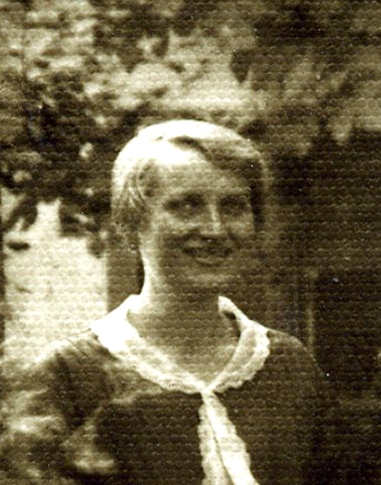
\includegraphics[width=0.4\textwidth]{photo/anastazja_swierczynska_1.jpg}
\caption{Anastazja Świerczyńska}
\label{rys:anastazja_swierczynska_1}
\end{center}
\end{figure}

Nazywana była Hyjką, bo tak ją nazwał jej starszy o dwa lata braciszek Karlik, który nie mogąc sobie poradzić z trudnym dla niego zdrobnieniem imienia Anastazja – ,,Stazyjka'' uprościł je sobie do postaci ,,Hyjka''. I tak już zostało. Nasza stryjenka Anastazja po ukończeniu szkoły podstawowej w Łagiewnikach Wielkich uczyła się szyć u sióstr służebniczek śląskich w Lubecku. Tam też poczuła ducha powołania do stanu zakonnego. Wypracowawszy więc sobie na służbie, jako niańka u Wincentego i Jadwigi Grabińskich (Wincenty był bratem naszej babci Eufemii), wymagane przez klasztor wiano, \textbf{wstąpiła 29 grudnia 1934 r. do Zgromadzenia Sióstr Służebniczek Najświętszej Maryi Panny Niepokalanie Poczętej}, które Dom Prowincjalny ma w Katowicach przy ul. Panewnickiej 63 – sąsiadujący z bazyliką franciszkańską p.w. św. Ludwika Króla. \textbf{5 stycznia 1937 r. złożyła pierwsze śluby, a 19 grudnia 1942 r. śluby wieczyste}. Tak swą starszą o dziesięć lat siostrę wspomina jej brat Benedykt: Anastazja, to jest ,,Hyjka'' była bardzo spokojna, posłuszna Mamie, bardzo dbała o czystość w domu, zawsze o czymś dumała głęboko, była raczej smutna.
\begin{figure}[!h]
\begin{center}
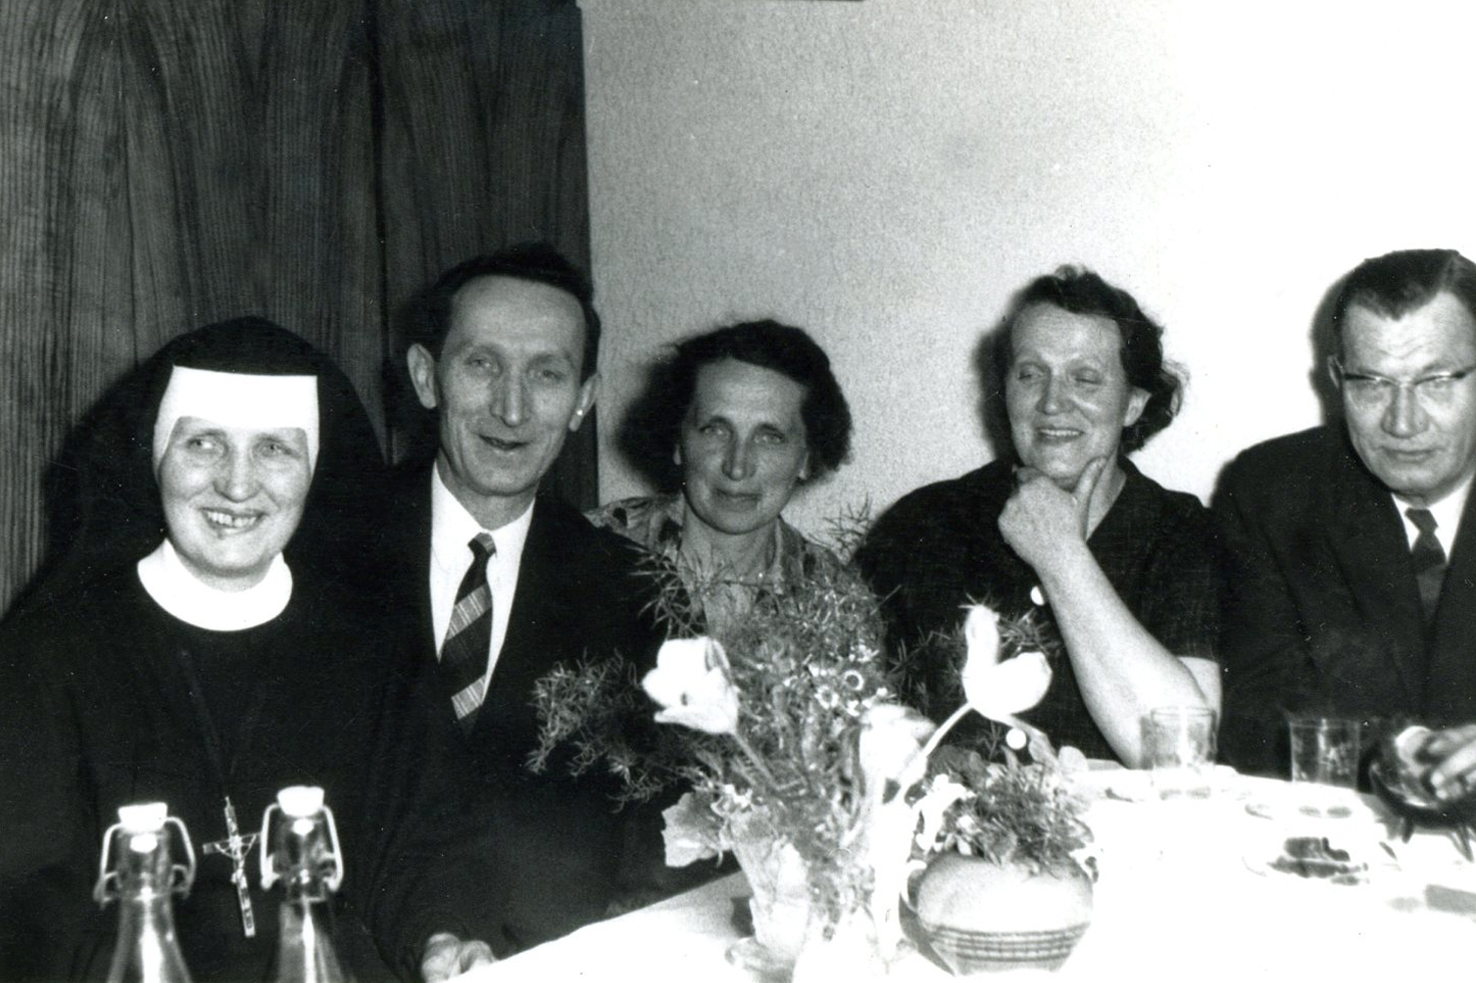
\includegraphics[width=0.65\textwidth]{photo/anastazja_swierczynska_2.jpg}
\caption[Anastazja Świerczyńska z rodzeństwem]{Anastazja Świerczyńska z rodzeństwem. Na zdj. od lewej: Anastazja Aurelia Świerczyńska, Benedykt Świerczyński, Róża Kuś, Irena Lehman i Józef Świerczyński.}
\label{rys:anastazja_swierczynska_2}
\end{center}
\end{figure}
\begin{figure}[!h]
\begin{center}
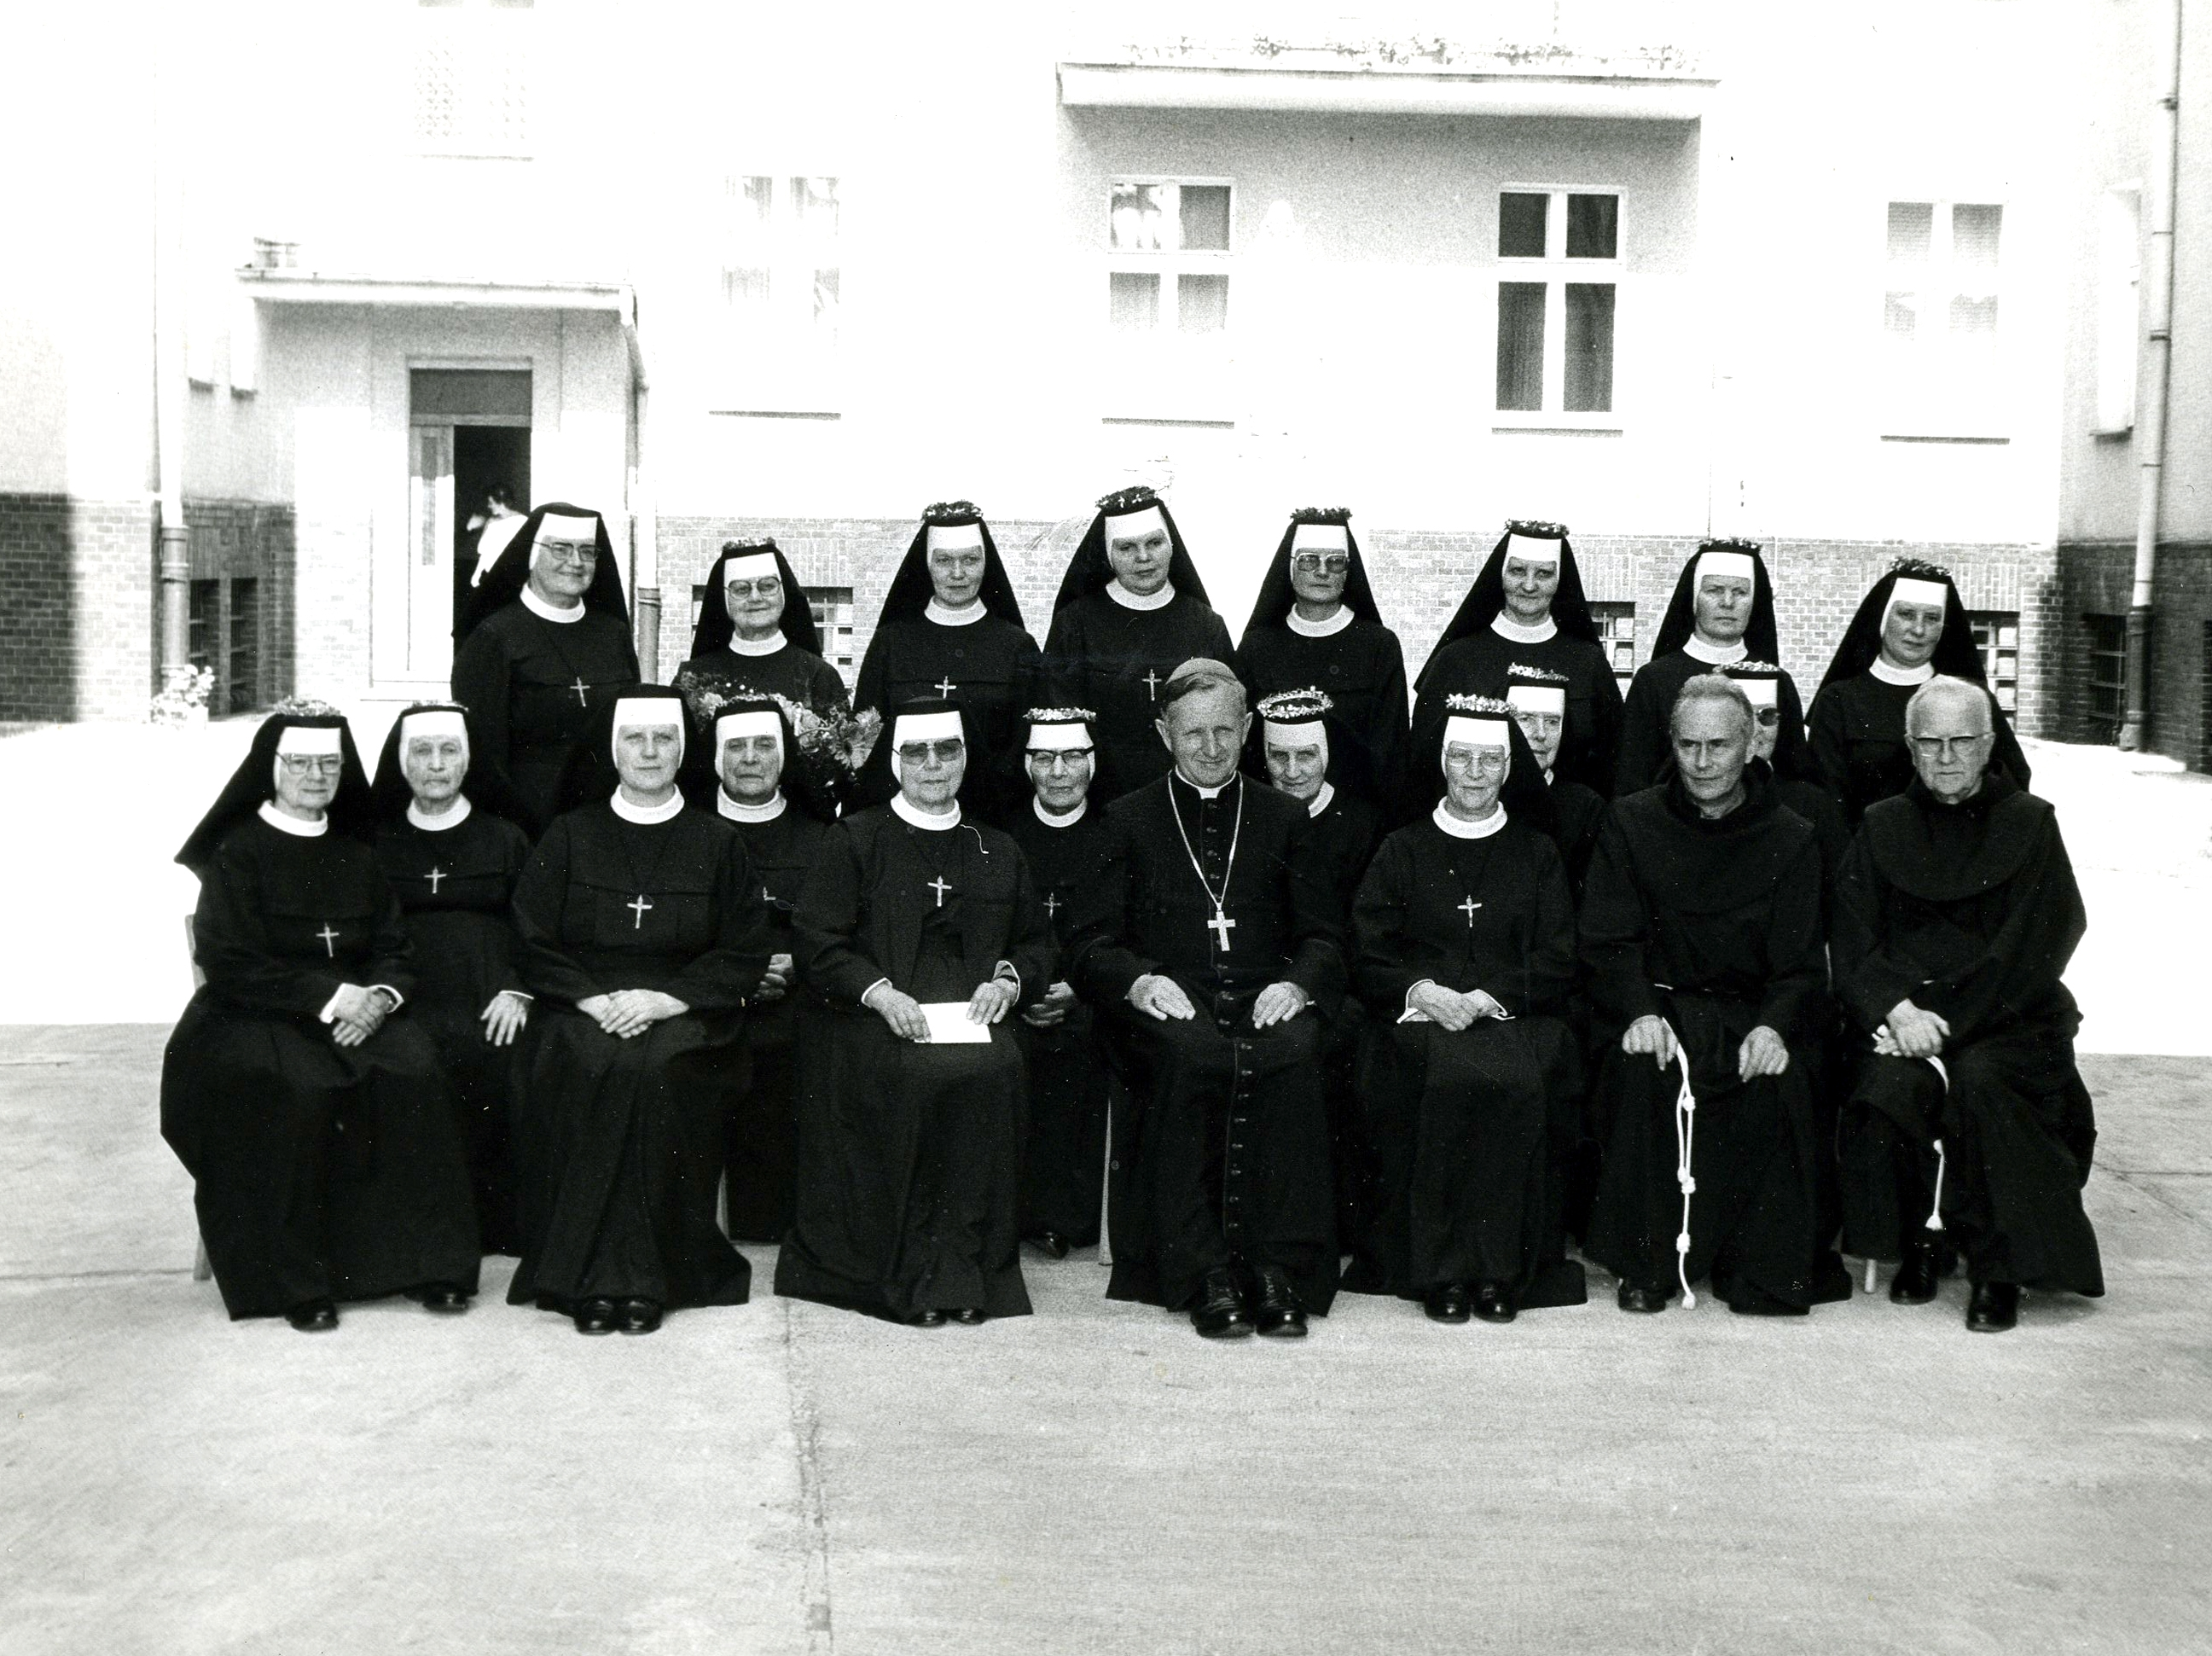
\includegraphics[width=0.8\textwidth]{photo/anastazja_swierczynska_3.jpg}
\caption[Siostra Anastazja z biskupem Zimoniem]{Siostra Anastazja z biskupem Zimoniem (zaraz za nim od prawej)}
\label{rys:anastazja_swierczynska_3}
\end{center}
\end{figure}

\begin{figure}[!b]
\begin{center}
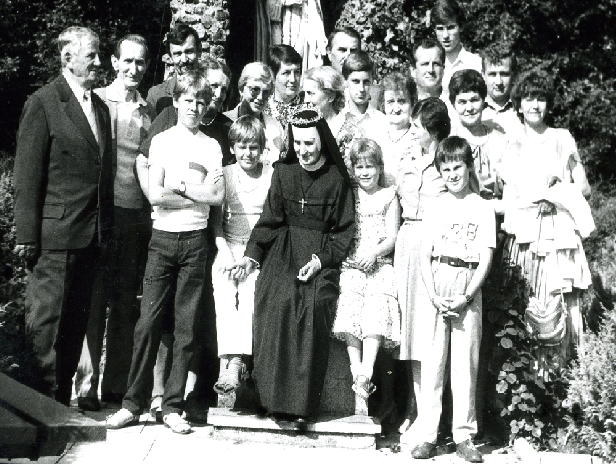
\includegraphics[width=0.7\textwidth]{photo/anastazja_swierczynska_4.jpg}
\caption[Jubileusz siostry Aurelii Anastazji Świerczyńskiej]{Jubileusz siostry Aurelii Anastazji Świerczyńskiej. Na zdj. od lewej stoją: Teodor Kuś, Benedykt Świerczyński, Czesław Świerczyński, przed nim Róża Kuś z Arturem Kusiem. Przed nimi siedzą: Marcin Kuś i Kasia Lehman z Jubilatką. Za nią stoją: Regina i Marysia Kuś oraz Irena Lehman. Obok niej stoi Krzysiu Lehman, a za nim jego ojciec - Tadeusz Lehman. Obok i za Kasią Lehman stoi babcia Radinka, za nią Edward Kuś, a za nim Tomasz Lehman. Obok Babci stoi Lubomira Lehman (żona Tadeusza), za nią Izydor Kuś, obok Lubomiry Marta Lehman. Przed nimi stoi Michał Lehman (brat Kasi, syn Bogusia). Obok babci Radinki czyżby stała Zuzia?}
\label{rys:anastazja_swierczynska_4}
\end{center}
\end{figure}

W 1939 roku ukończyła Szkołę Pielęgniarską w Poznaniu -- wysłana tam przez siostrę przełożoną. Praktykę odbywała w szpitalu w Katowicach, zaś Niemcy przenieśli ją wraz z innymi siostrami do szpitala w Zabrzu, gdzie pracowała do końca wojny. W latach 1945~-~49 była pielęgniarką w Chełmie Wielkim. Potem pracowała w charakterze instrumentariuszki w Sali operacyjnej w szpitalu w Chorzowie, następnie została przełożoną Domu Małego Dziecka w Rybniku, który pewną ręką prowadziła w latach 1950~-~57. Wtedy to odwiedziła nas (mnie i mojego brata -- Józia) w szpitalu zakaźnym (byliśmy chorzy na szkarlatynę), do którego nikt – poza służbą medyczną (nie wyłączając rodziców) nie miał wstępu. Jakaż to była radość po wielu dniach samotności i obcości widzieć swojską, bliską sercu twarz! Z Rybnika przełożona przeniosła ją jako pielęgniarkę szczególnie kompetentną i odpowiedzialną do Sanatorium Przeciwgruźliczego w Istebnej, gdzie ofiarnie służyła w latach 1957~-~1964.

W latach 1971~-~1974 była przełożoną w klasztorze we Wrocławiu przy ul. Łaciarskiej. Po tym trudnym doświadczeniu prowadzenia całego Domu wróciła do siebie, tzn. na Panewnicką 63, do Domu Prowincjalnego, gdzie była cenioną hafciarką. I tak już niemal do końca życia, póki wzrok pozwalał, lecz w Domu Świętej Anny -- vis a vis Domu Prowincjalego, gdzie \textbf{doczekała w 1987 r. wspaniałego Jubileuszu 50-lecia od złożenia pierwszej profesji!} 

I ja tam byłem wraz z całą niemal rodziną Świerczyńskich\ldots

Wielki, dobroczynny wpływ wywarła stryjenka Anastazja na życie swej o 7 lat młodszej siostry Ireny. Najpierw wysłała ją do dwuletniej Państwowej Szkoły dla Położnych w Chorzowie (stryjenka Irena doczekała w tym zawodzie emerytury jako niezwykle ceniona akuszerka).
\begin{figure}[!h]
\begin{center}
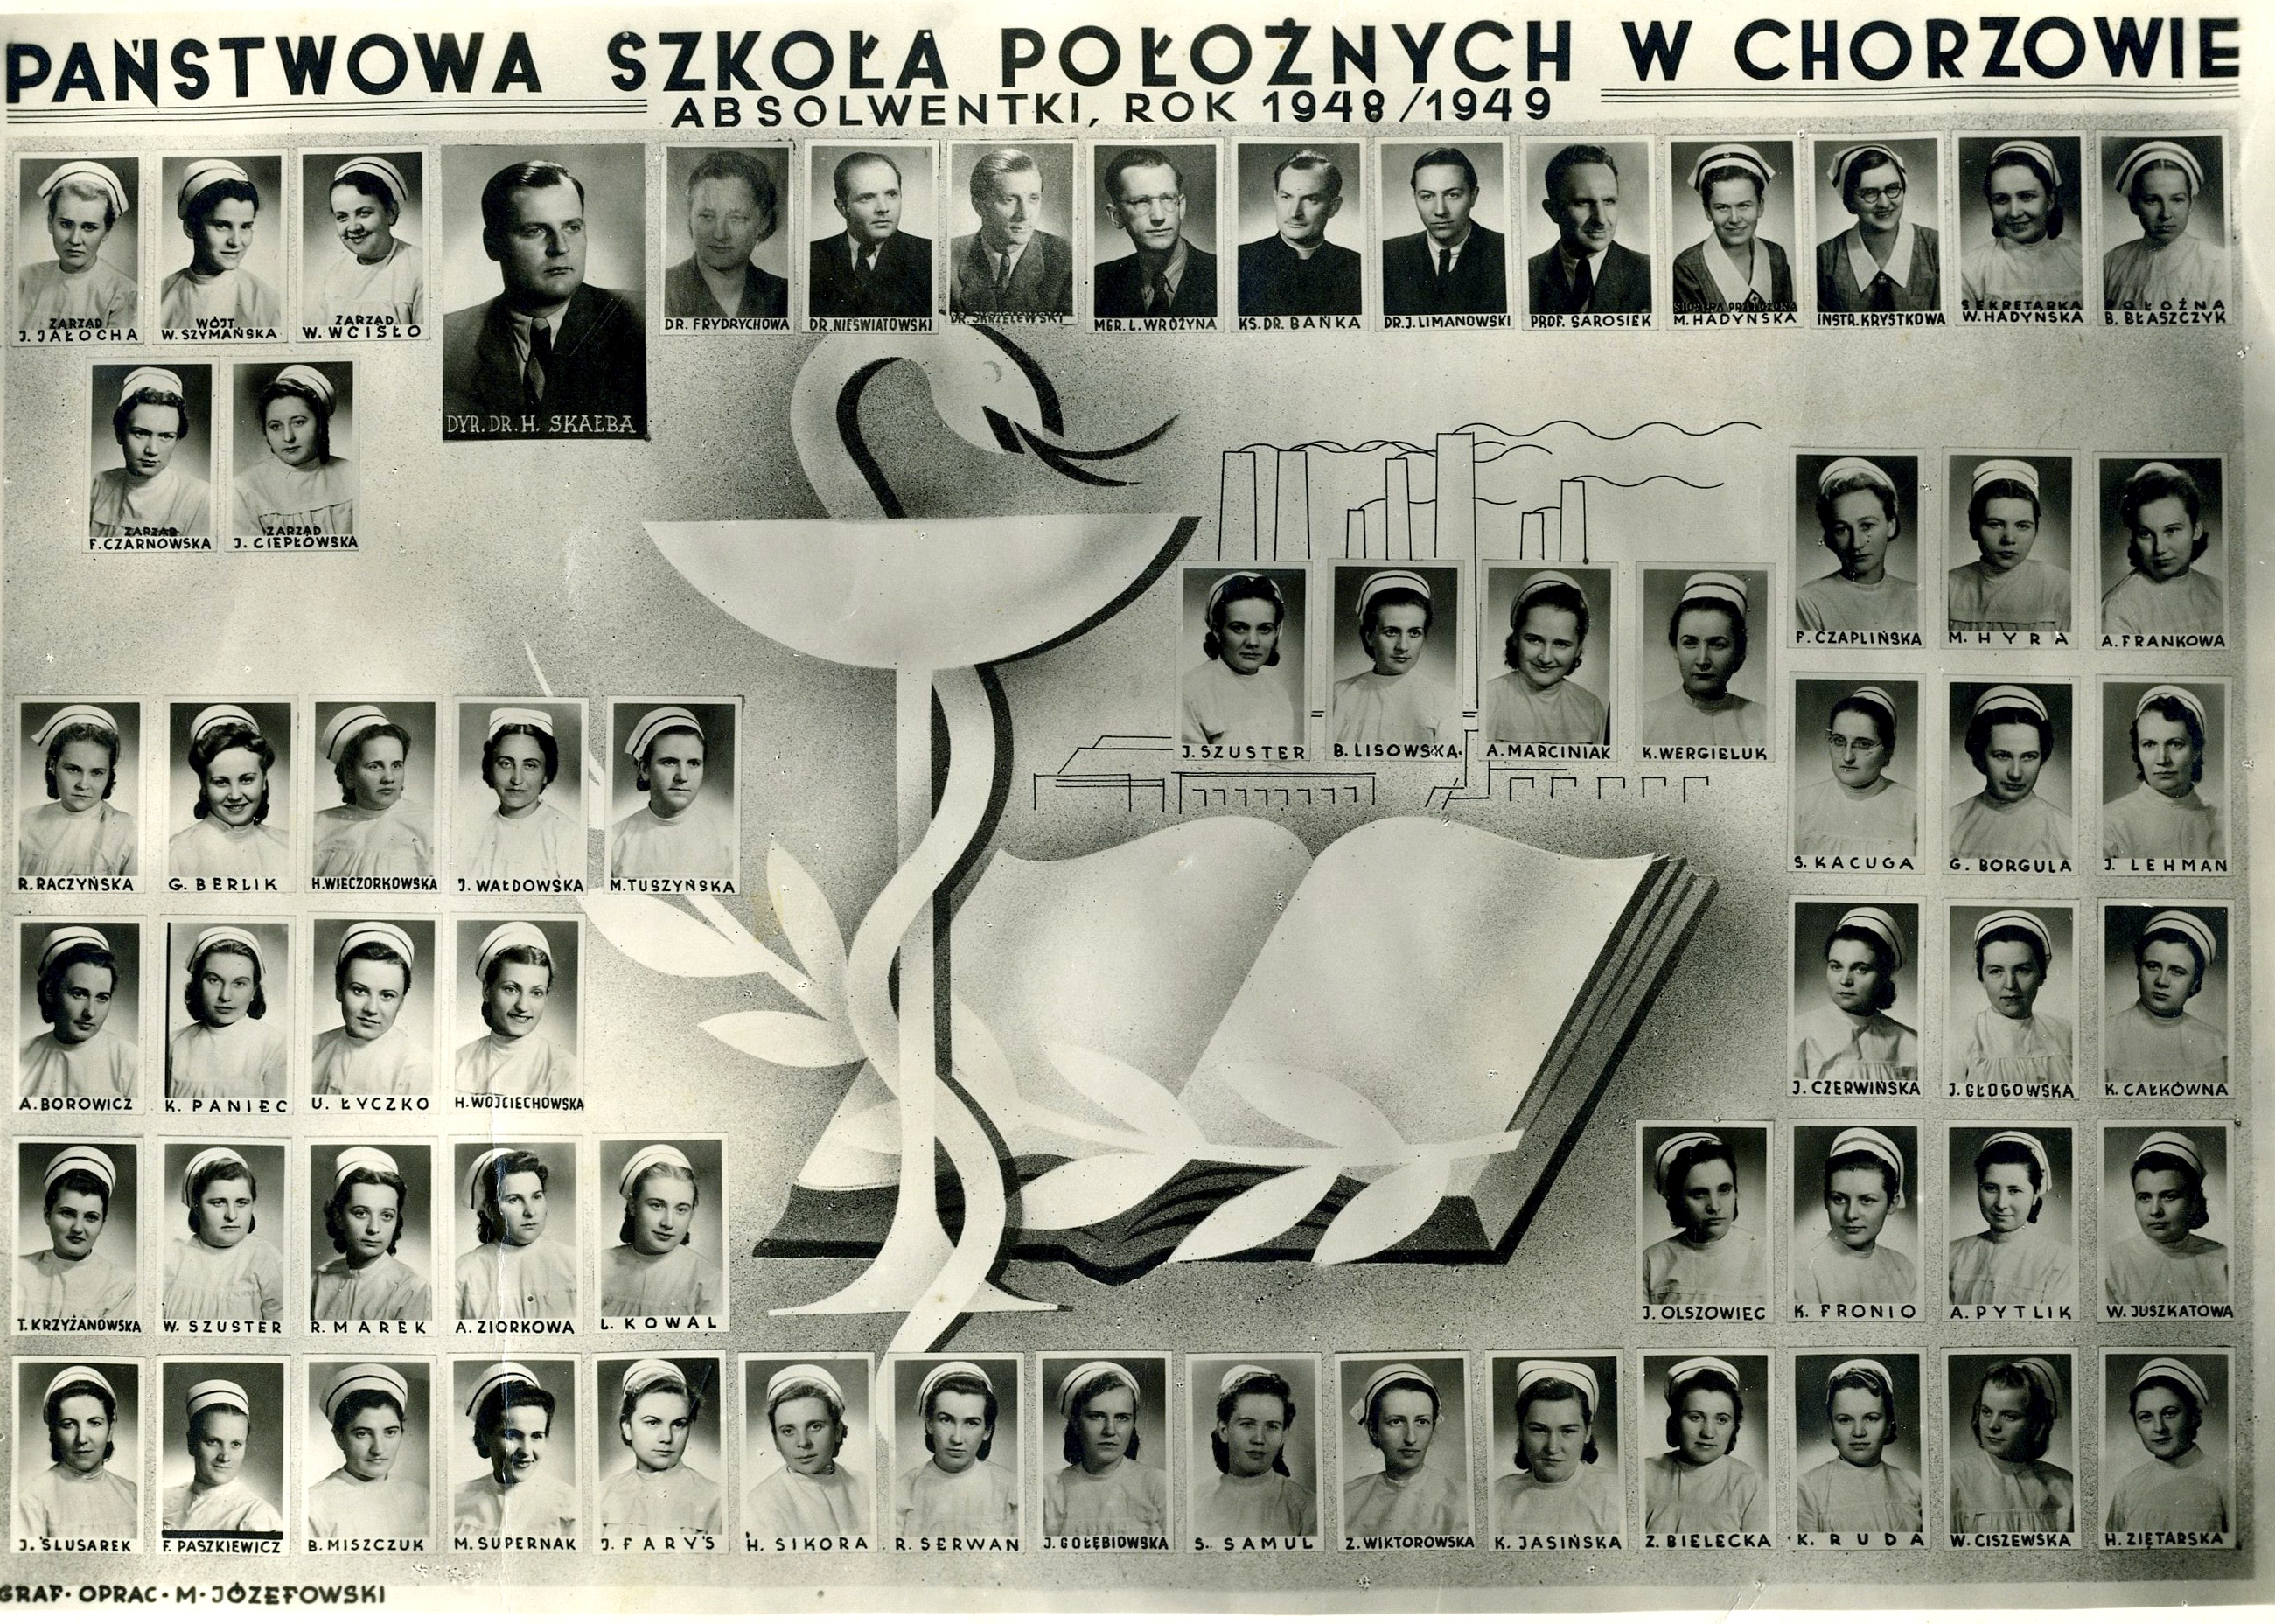
\includegraphics[width=\textwidth]{photo/szkola_poloznych_w_chorzowie.jpg}
\caption[Absolwentki Państwowej Szkoły Położnych w Chorzowie.]{Absolwentki Państwowej Szkoły Położnych w Chorzowie. Na zdj. stryjenka Irena w skrajnym prawym rzędzie druga od góry.}
\label{rys:szkola_poloznych_w_chorzowie}
\end{center}
\end{figure}

\begin{figure}[!h]
\begin{center}
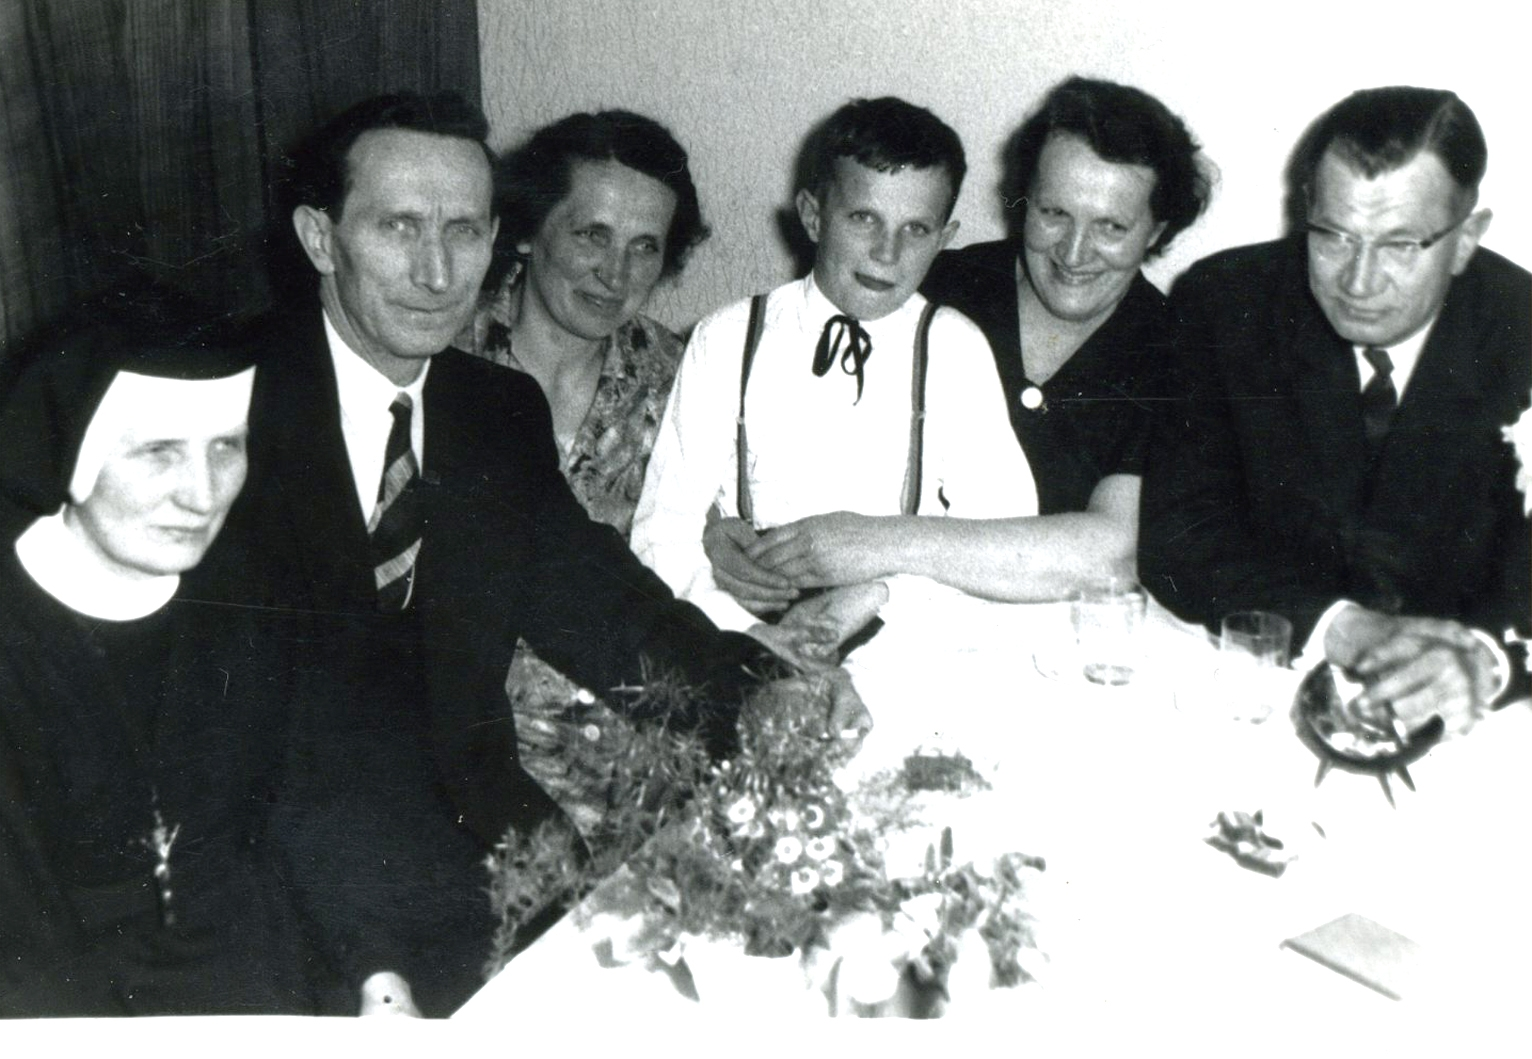
\includegraphics[width=0.85\textwidth]{photo/anastazja_swierczynska_5.jpg}
\caption[Rodzeństwo Świerczyńskich]{Na zdj. od lewej Anastazja Świerczyńska, Benedykt Świerczyński, Róża Kuś, Boguś Lehman (najmłodszy syn Ireny) Irena Lehman i Józef Świerczyński.}
\label{rys:anastazja_swierczynska_5}
\end{center}
\end{figure}

Gdy zaś jej mąż -- stryj Antoni znalazł się w więzieniu, a ona chciała być blisko męża, siostra Stazyjka i jednocześnie siostra siostry zakonnej – Celiny Miodek znalazły dla niej mieszkanie w Gdańsku Wrzeszczu u Klary Miodek – siostry Celiny, przy ul Dzielnej 21.

Zawsze ciepło wypowiadała się o swoich bliskich, zwłaszcza o naszym Tacie, ubolewając jednocześnie, że tak wiernie służy wrogiej Kościołowi Katolickiemu – ideologii. I zawsze uczestniczyła we wszystkich ważnych uroczystościach rodzinnych w stroju zakonnym (który nawiasem mówiąc też się nieznacznie zmieniał, stając się, oględnie mówiąc, coraz mniej ostentacyjny).

Pod koniec Jej życia odwiedziłem kilka razy kochaną stryjenkę w Domu Św. Anny, gdzie zawsze byłem przyjmowany z wielką radością i bardzo wylewnie. \textbf{Zmarła 16 Listopada 1993~r. w~Domu Św. Anny w Katowicach Panewnikach, opatrzona, ma się rozumieć, świętymi sakramentami.}